\chapter{Results}
\label{chapter:Results}

\section{Using graph convolution in the way it's meant to be used gives poor results on molecular structures}


\begin{figure}[H]
	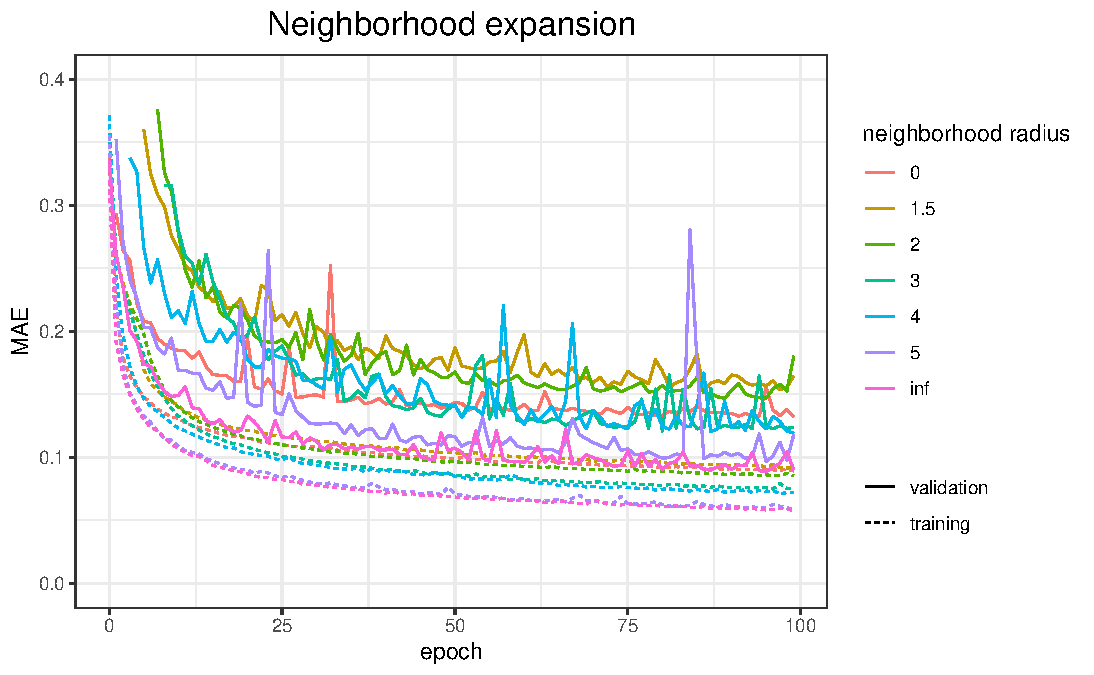
\includegraphics[width=\linewidth]{figures/tencent-mpnn-neighborhood-expansion}
	
	\caption{some caption...}
	\label{fig:distance_threshold}
\end{figure}

{\itshape

Show that, for decreasing thresholds, performance decreases

Emphasize that this is not really appreciated in the literature.
Cite Alchemy paper and point out that the high-performing kaggle-teams all use fully connected graphs.
Does no one notice?

Repeat that the conv should be able to handle this because after several MP steps, the effective field of vision is the entire molecule - but it doesn't work well
}

\section{Introducing a graph-state at every graph-conv layer improves results}



{\itshape
explain hypothesis:
lack of information of global environment. Maybe graph-level features needed at every conv?

Test this hypothesis:
add graph-state
show figure: now the effect is less pronounced because the global environment is accessible through the graph-state

Why this is important:
in larger graphs the option of using a fully connected graph is simply not there:
show computational complexity graph
}


\section{graph-conv layers with independent weights do not improve results}

{\itshape
	
OPTIONAL SECTION

It's reasonable to assume, that different layers need different feature extraction properties (low vs. high level features). In cv, the layers don't share weights.

However, in experiments, the weight-shared graph layers prove superior.
}

\section{relative position edge features improve results slightly}

{\itshape
 Show that relative position edge features slightly improve the results but not much
 
 explain that the problem is probably that they are not rotation-invariant
	
	
OPTIONAL PART:\\
review the results of the 3DGCN-paper and show that this doesn't work really well on the Alchemy data - probably for the same reason given above
}

Citation is all you need~\cite{Vaswani2017}





